\section{Resultados e Discussão}
\label{chap:resultados}

A investigação empírica dos quatro métodos manuais para estimação da matriz de covariância foi estruturada para responder a questões sobre eficiência computacional, precisão numérica e estabilidade em cenários de alta dimensionalidade. A Tabela~\ref{tab:benchmarks} apresenta os tempos de execução médios, evidenciando a superioridade das implementações vetorizadas (\texttt{mcovar2} e \texttt{mcovar4}) em relação às versões baseadas em laços explícitos (\texttt{mcovar1} e \texttt{mcovar3}).

\begin{table}[h]
\centering
\caption{Benchmarks de tempo de execução (Média $\pm$ Desvio Padrão em ms) para 100 rodadas.}
\label{tab:benchmarks}
\resizebox{\columnwidth}{!}{%
\begin{tabular}{l|rr|rr}
\toprule
 & \multicolumn{2}{c|}{\textbf{4 Sensores}} & \multicolumn{2}{c}{\textbf{24 Sensores}} \\
\textbf{Método} & \textbf{Média (ms)} & \textbf{Desvio (ms)} & \textbf{Média (ms)} & \textbf{Desvio (ms)} \\
\midrule
\texttt{mcovar1} (Loop-Dev) & $14{,}62$ & $0{,}05$ & $18{,}84$ & $0{,}10$ \\
\texttt{mcovar2} (Matriz-Dev) & $0{,}04$ & $0{,}00$ & $0{,}20$ & $0{,}01$ \\
\texttt{mcovar3} (Loop-Mom) & $14{,}73$ & $0{,}07$ & $19{,}27$ & $0{,}11$ \\
\texttt{mcovar4} (Matriz-Mom) & $\mathbf{0{,}04}$ & $0{,}01$ & $\mathbf{0{,}17}$ & $0{,}01$ \\
\texttt{NumPy Cov} & $0{,}06$ & $0{,}01$ & $0{,}32$ & $0{,}01$ \\
\bottomrule
\end{tabular}%
}
\end{table}

As implementações matriciais demonstraram ser ordens de magnitude mais rápidas que as versões com laço ($\sim 500\times$ mais rápidas para 4 sensores e $\sim 100\times$ para 24 sensores). O método \texttt{mcovar4} apresentou o melhor desempenho geral, superando inclusive a função nativa do NumPy em ambos os cenários de dimensionalidade. Esta diferença de desempenho ocorre porque a implementação manual via momentos de segunda ordem minimiza as checagens de tipos e tratamentos genéricos de NaNs que o \texttt{np.cov} realiza por padrão. A Figura~\ref{fig:benchmark_plots} ilustra graficamente estas discrepâncias através de histogramas e \textit{violin plots} que evidenciam a baixa variância e alta eficiência dos métodos vetorizados.

\begin{figure}[h]
    \centering
    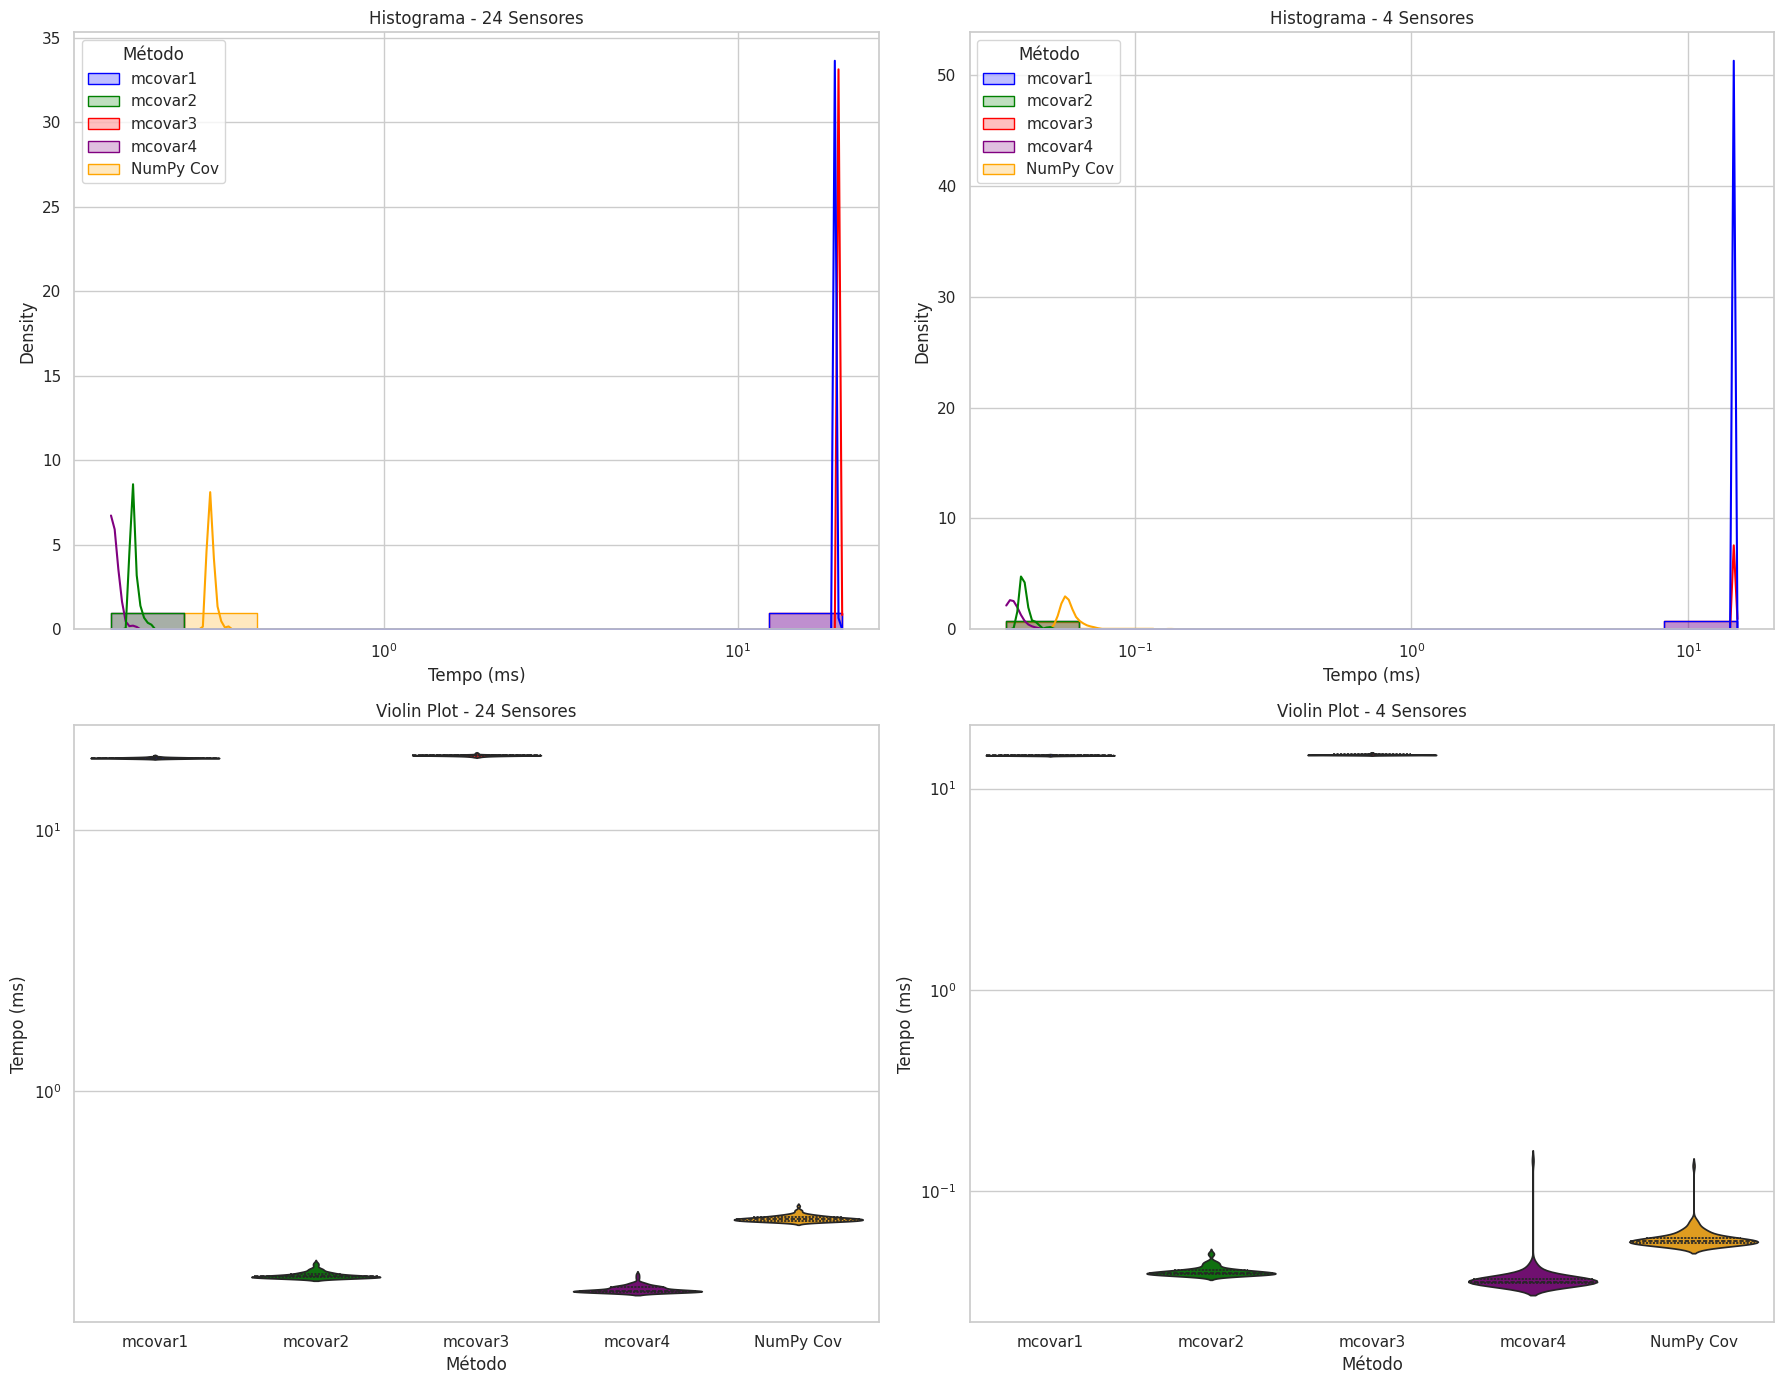
\includegraphics[width=0.9\textwidth]{figuras/benchmark_plots.png}
    \caption{Distribuição de tempos de execução (Histograma e Violin Plot) para os métodos manuais vs NumPy Cov. A escala logarítmica evidencia a separação entre abordagens vetorizadas e baseadas em laços.}
    \label{fig:benchmark_plots}
\end{figure}

Em termos de precisão numérica, todos os métodos produziram resultados estatisticamente indistinguíveis da referência do NumPy, com normas de Frobenius residuais da ordem de $10^{-4}$ a $10^{-3}$, inerentes às pequenas variações de arredondamento em ponto flutuante. A visualização das matrizes via mapas de calor (Figura~\ref{fig:heatmaps}) revela padrões claros de correlação entre os sensores adjacentes, confirmando a redundância espacial característica do robô \textit{Wall-Following}.

\begin{figure}[h]
    \centering
    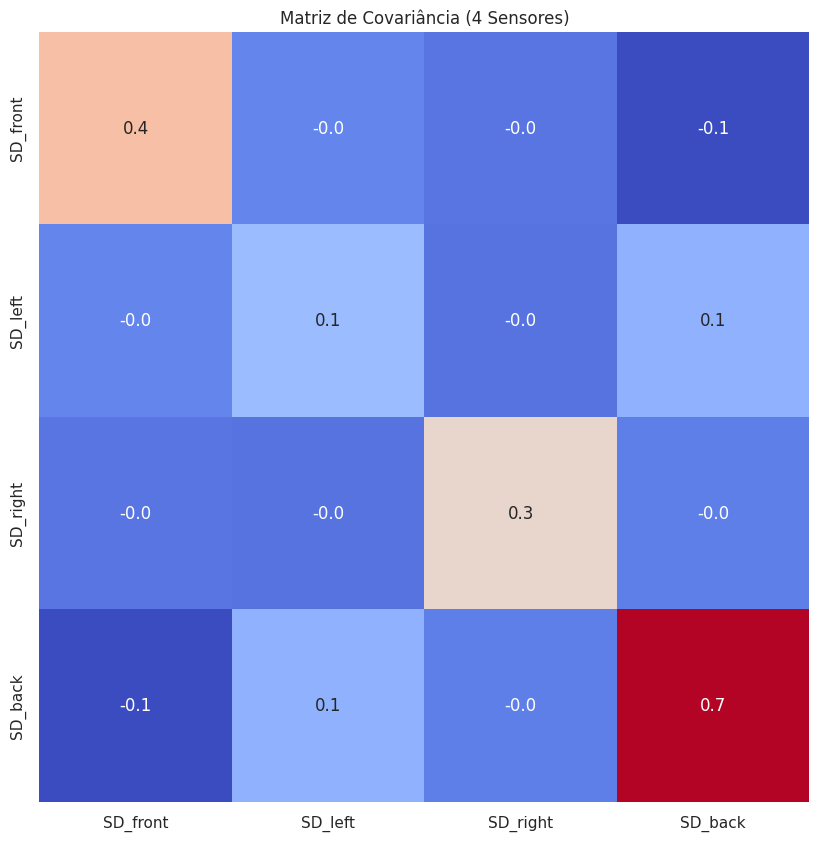
\includegraphics[width=0.8\textwidth]{figuras/heatmap_cov_4.png}
    \caption{Mapas de calor das matrizes de covariância para os cenários de 4 e 24 sensores. Nota-se a alta covariância positiva entre sensores adjacentes, indicando redundância de sinal.}
    \label{fig:heatmaps}
\end{figure}

Um ponto crítico revelado na análise foi a falta de posto completo nas matrizes originais. Para o cenário de 24 sensores, o posto observado foi consistentemente $Rank = 23$, indicando que ao menos um sensor é linearmente dependente dos demais. O número de condicionamento extremamente elevado ($> 10^{20}$) inviabiliza a inversão direta de $\mathbf{C}$ para fins de classificação. Para contornar esta singularidade, a regularização de Tikhonov ($\mathbf{C} + 0{,}1\mathbf{I}$) foi aplicada com sucesso, restaurando o posto completo e garantindo a estabilidade numérica dos modelos probabilísticos subsequentes, sem perda significativa de informação estrutural.
